\appendix
\chapter*{Annexes}

\section{Liens vers les notebooks Colab et GitHub}

\begin{itemize}
  \item \href{https://colab.research.google.com/drive/1WhaF2jE4ruWc6pByavec3E4Q6ijtsSvc?usp=sharing}{Colab d'entraînement du modèle de régression}

  \item \href{https://colab.research.google.com/drive/1iKeuTVjw6RtWP935TcWio7b9p6vjdsI0?usp=sharing}{Colab d'entraînement du modèle de classification}

  \item \href{https://colab.research.google.com/drive/1MJzRelOdtMpLDED62YKCTAENZ-j5BKGF?usp=sharing}{Colab de prétraitement de données pour la classification}

  \item Colab de prétraitement de données pour la régression : 
  \begin{itemize}
    \item \href{https://colab.research.google.com/drive/1aUlAik45c6v8C0GXGo_OrgLEPCQ-7mMI?usp=sharing}{Notebook 1}
    \item \href{https://colab.research.google.com/drive/1Xe0IfXKSYyPatz7qS6MPJhF55g3mx633?usp=sharing}{Notebook 2}
  \end{itemize}

  \item \href{https://github.com/Thisi47/bean_cooking_time_predictor.git}{GitHub de l'application Android}
\end{itemize}


Dans le but de valider l’intégration du modèle sur l’application Android, nous présentons ci-après un ensemble d’images de test capturées sur l’appareil, illustrant la performance et la cohérence des prédictions obtenues.

\begin{figure}[H]
    \centering

    % Ligne 1
    \begin{subfigure}{0.2\textwidth}
        \centering
        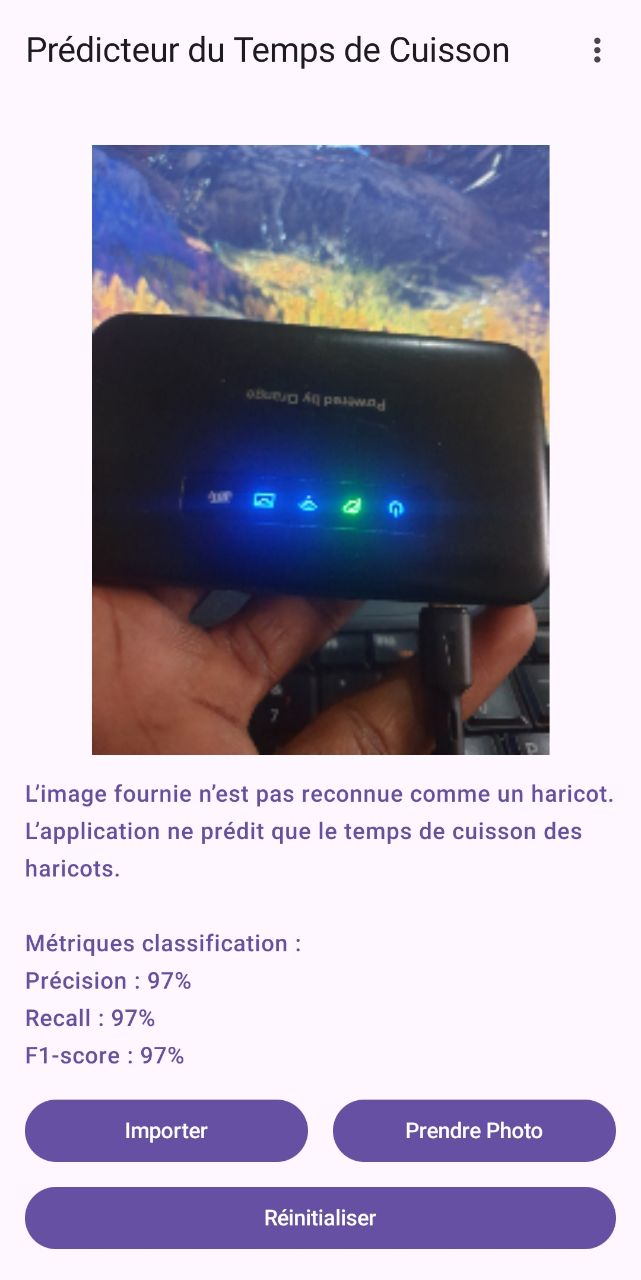
\includegraphics[width=\linewidth]{figures/test4.jpg}
        \caption{Image 4}
    \end{subfigure}\hfill
    \begin{subfigure}{0.2\textwidth}
        \centering
        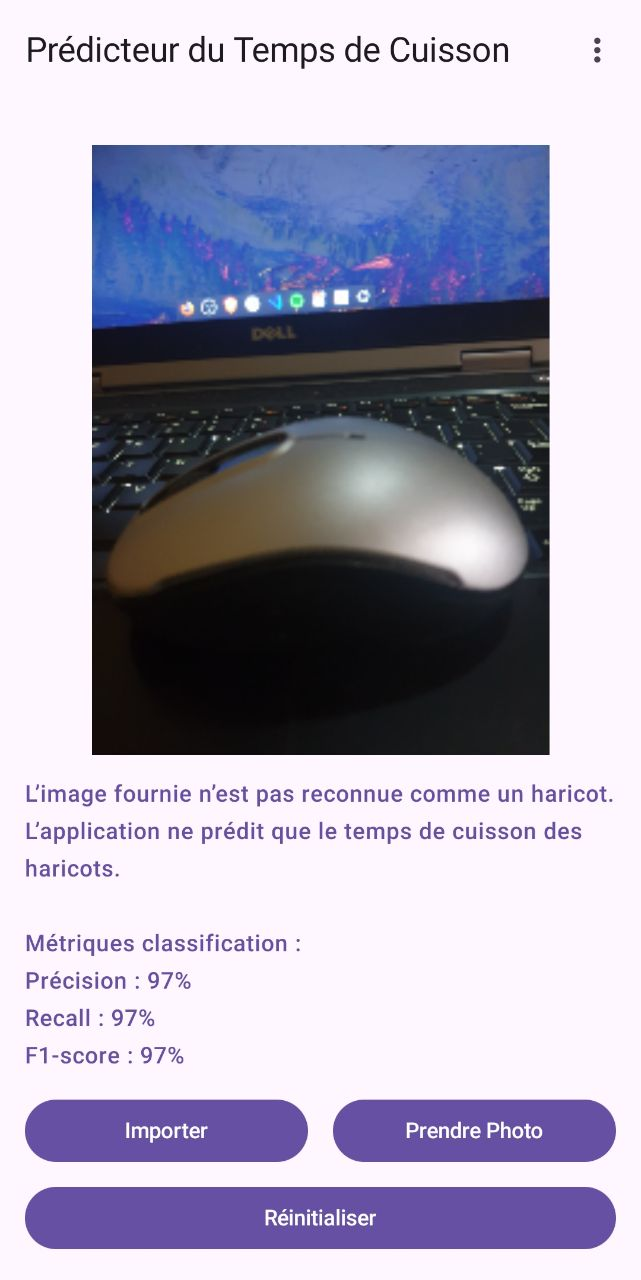
\includegraphics[width=\linewidth]{figures/test2.jpg}
        \caption{Image 2}
    \end{subfigure}\hfill
    \begin{subfigure}{0.2\textwidth}
        \centering
        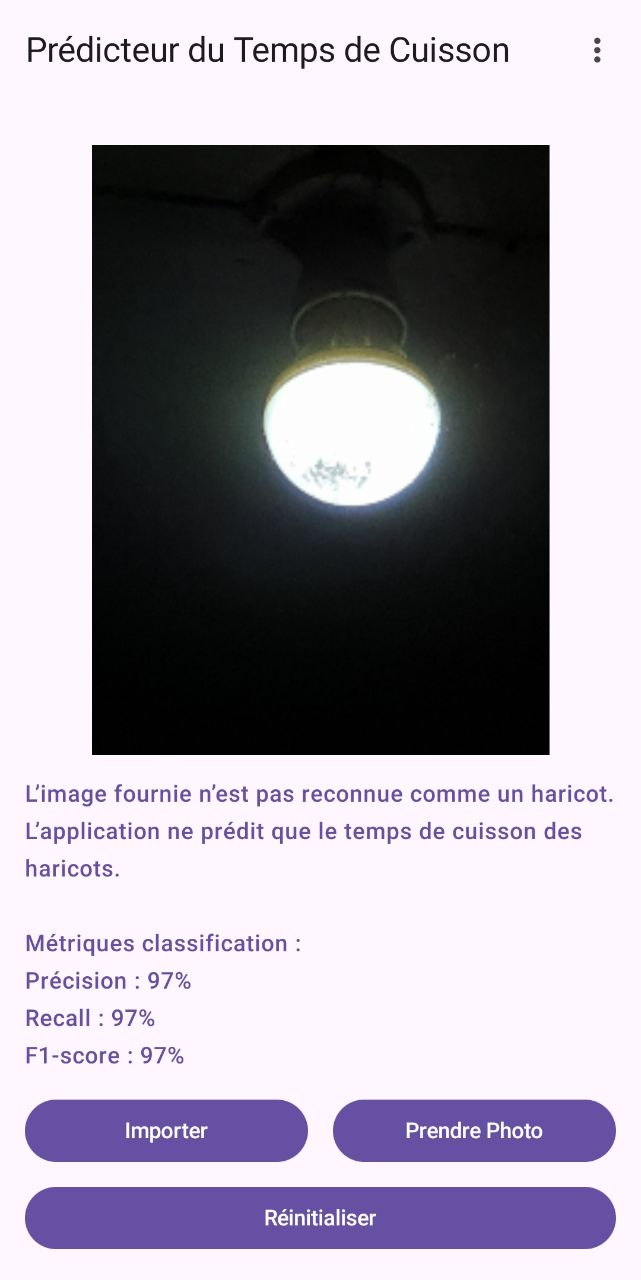
\includegraphics[width=\linewidth]{figures/test3.jpg}
        \caption{Image 3}
    \end{subfigure}

    % Ligne 2
    \begin{subfigure}{0.24\textwidth}
        \centering
        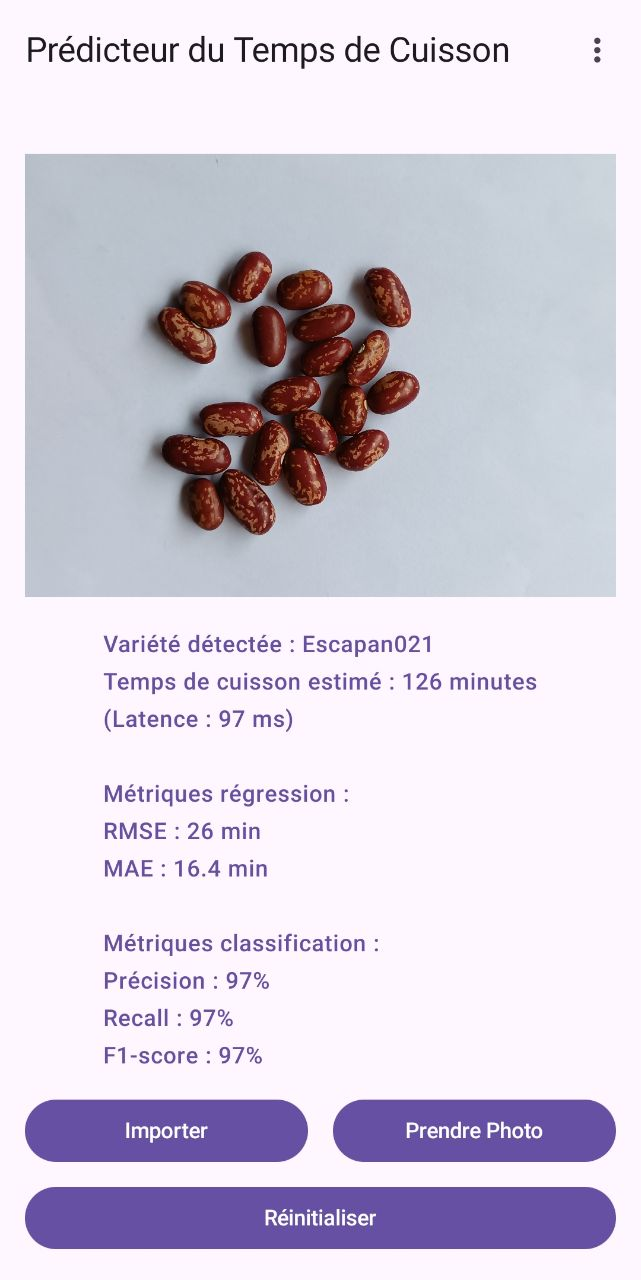
\includegraphics[width=\linewidth]{figures/test1.jpg}
        \caption{Image 1}
    \end{subfigure}\hfill
    \begin{subfigure}{0.24\textwidth}
        \centering
        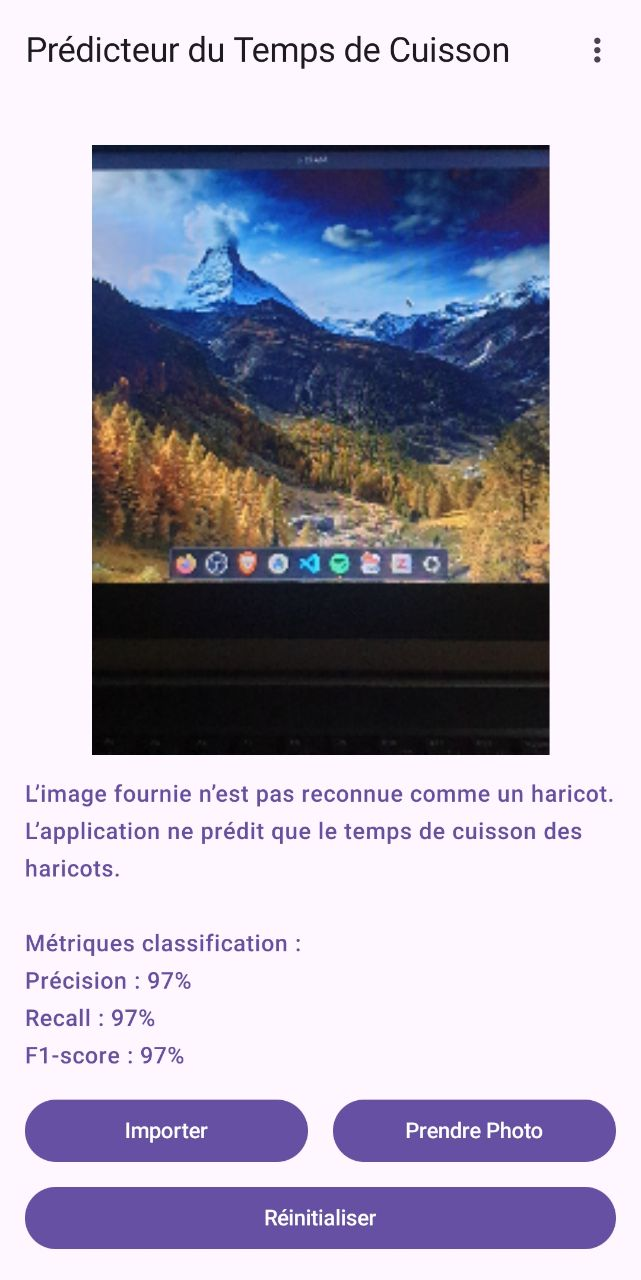
\includegraphics[width=\linewidth]{figures/test5.jpg}
        \caption{Image 5}
    \end{subfigure}\hfill
    \begin{subfigure}{0.24\textwidth}
        \centering
        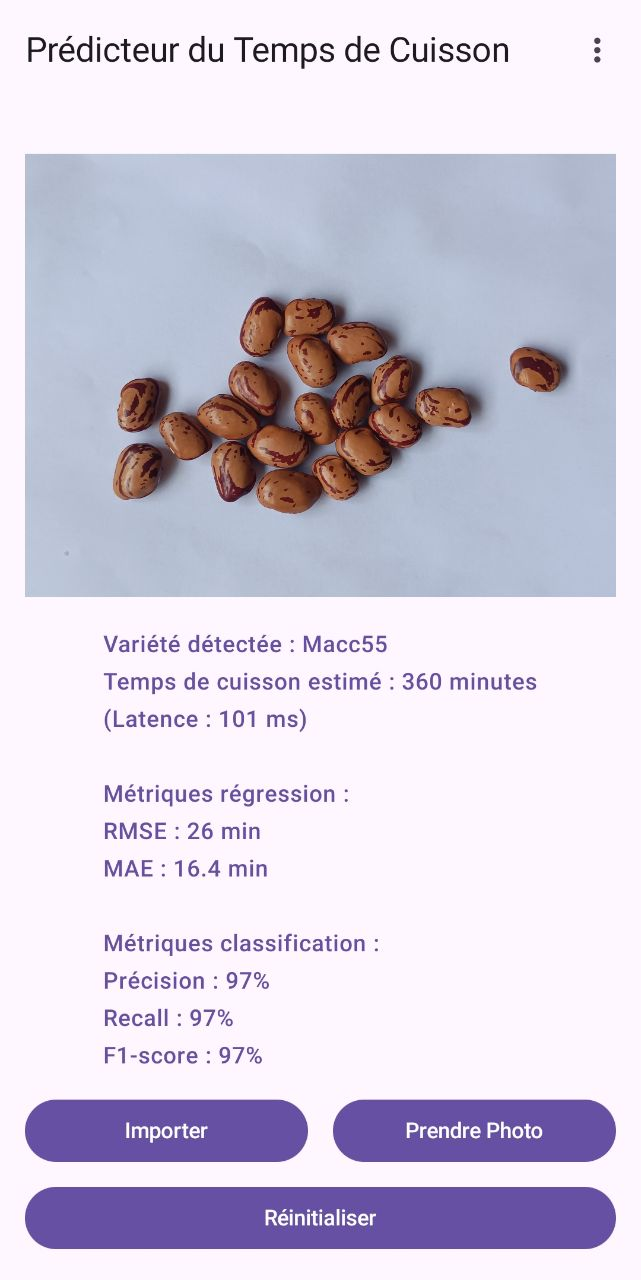
\includegraphics[width=\linewidth]{figures/test6.jpg}
        \caption{Image 6}
    \end{subfigure}

    % Ligne 3
    \begin{subfigure}{0.24\textwidth}
        \centering
        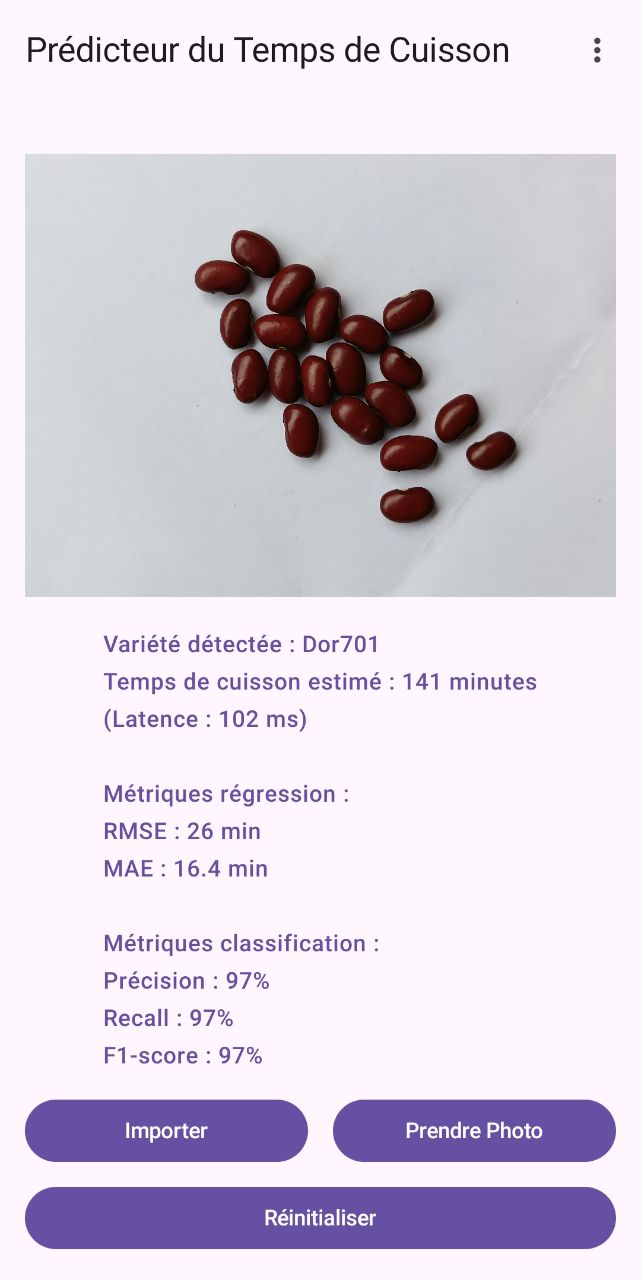
\includegraphics[width=\linewidth]{figures/test7.jpg}
        \caption{Image 7}
    \end{subfigure}\hfill
    \begin{subfigure}{0.24\textwidth}
        \centering
        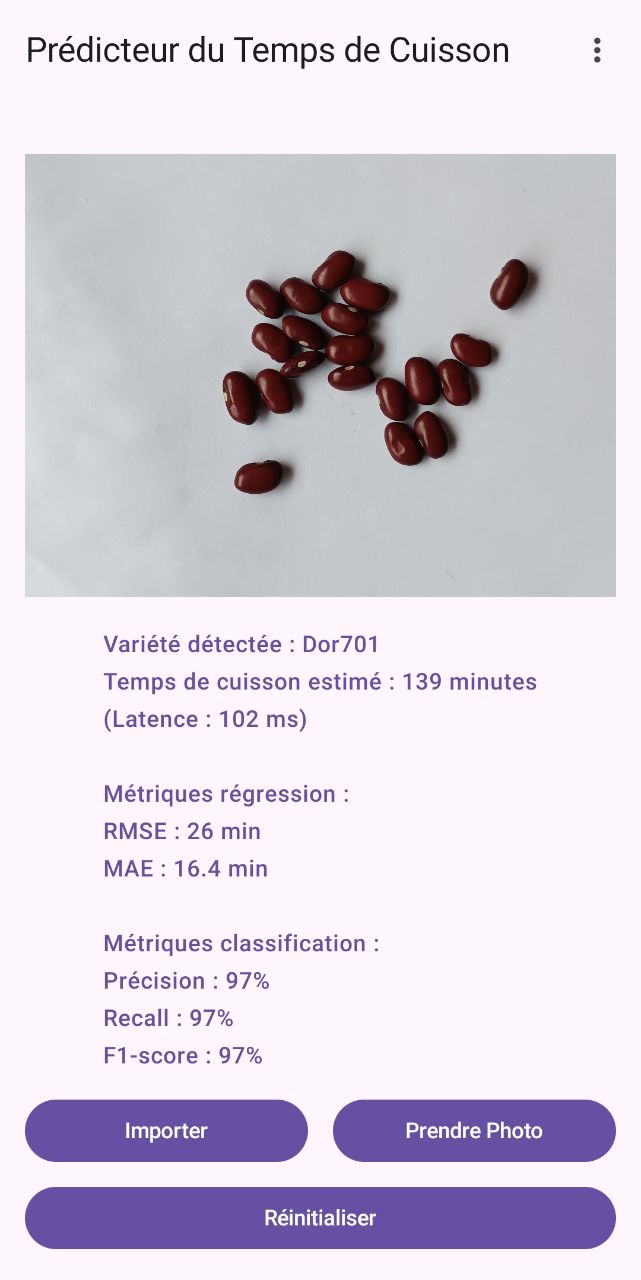
\includegraphics[width=\linewidth]{figures/test8.jpg}
        \caption{Image 8}
    \end{subfigure}\hfill
    \begin{subfigure}{0.24\textwidth}
        \centering
        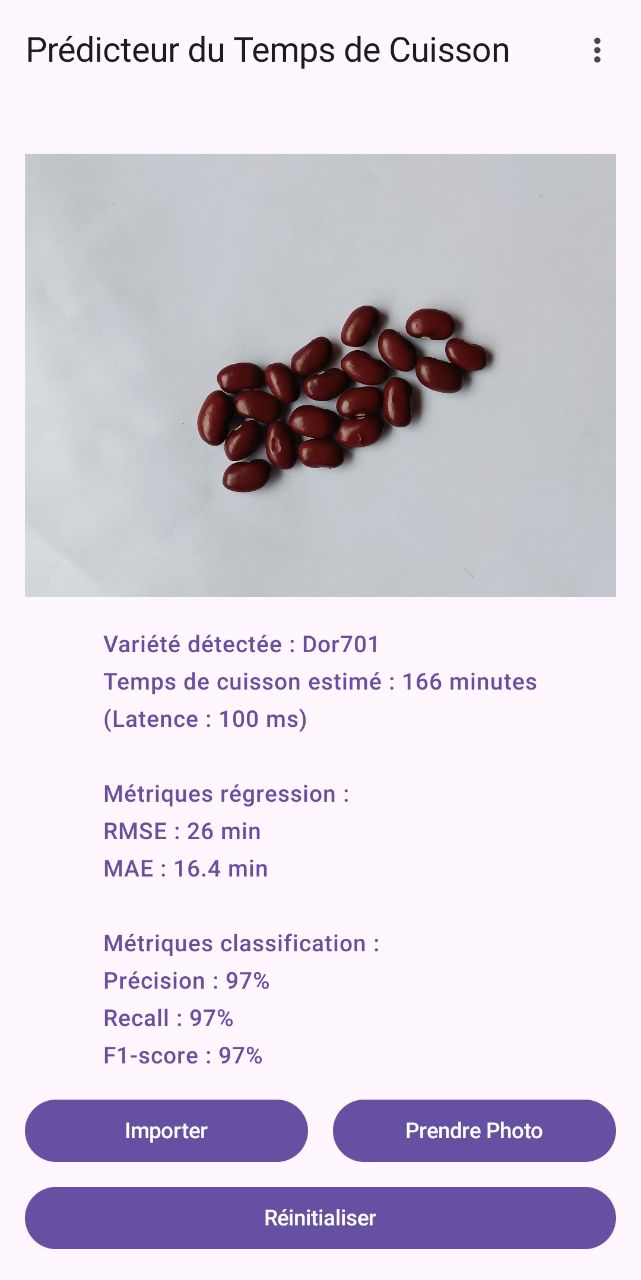
\includegraphics[width=\linewidth]{figures/test9.jpg}
        \caption{Image 9}
    \end{subfigure}

    % Ligne 4
    % \begin{subfigure}{0.3\textwidth}
    %     \centering
    %     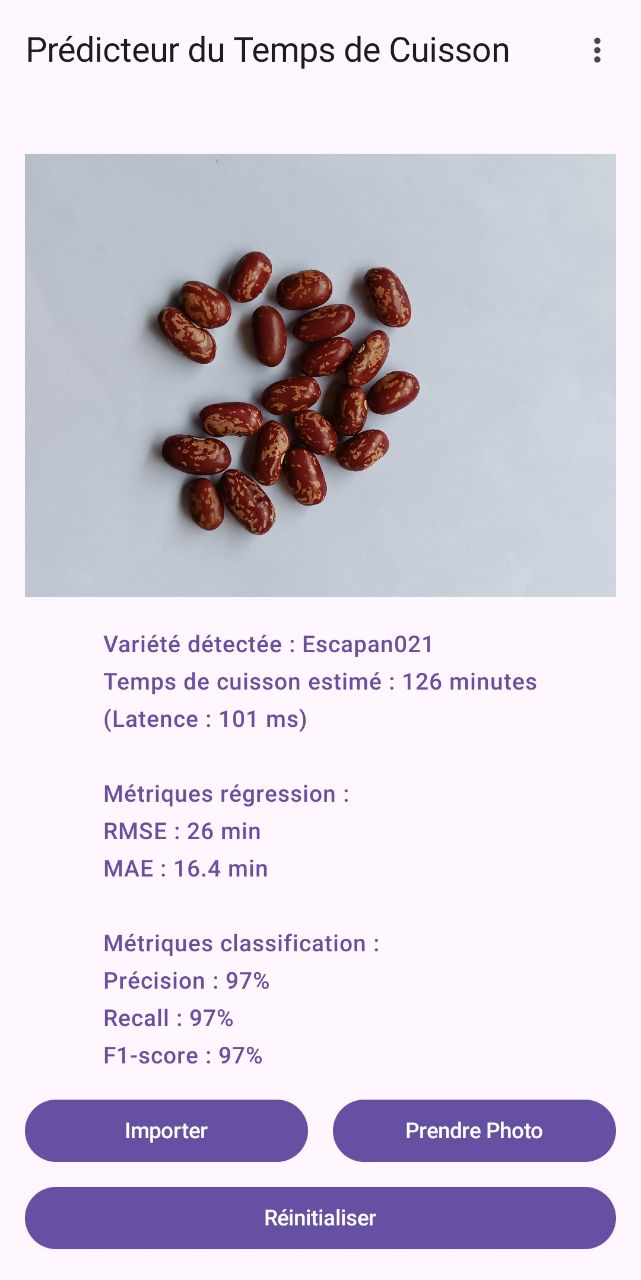
\includegraphics[width=\linewidth]{figures/test10.jpg}
    %     \caption{Image 10}
    % \end{subfigure}

    \caption{Images de test de l’application Android montrant les résultats de prédiction.}
    \label{fig:test_android}
\end{figure}
